\documentclass[aspectratio=169]{beamer}

% Show speaker notes on second screen for pympress
\usepackage{pgfpages}
% \setbeameroption{show notes on second screen=right}

% Match the existing CSE 534 Beamer styling
\usetheme{default}
\usecolortheme{default}
\setbeamertemplate{navigation symbols}{}
\setbeamertemplate{footline}[frame number]

\definecolor{darkbg}{HTML}{000000}
\definecolor{lighttext}{HTML}{999999}
\definecolor{miamired}{HTML}{941728}
\definecolor{codebg}{HTML}{1a1a1a}

\setbeamercolor{background canvas}{bg=darkbg}
\setbeamercolor{normal text}{fg=lighttext}
\setbeamercolor{frametitle}{fg=miamired}
\setbeamercolor{title}{fg=miamired}
\setbeamercolor{structure}{fg=miamired}
\setbeamercolor{item}{fg=miamired}
\setbeamercolor{block title}{fg=miamired,bg=codebg}
\setbeamercolor{block body}{fg=lighttext,bg=codebg}

\setbeamerfont{title}{series=\bfseries,size=\Large}
\setbeamerfont{frametitle}{series=\bfseries}

\usepackage{graphicx}
\usepackage{listings}
\usepackage{tikz}
\usepackage{array}
\usepackage{booktabs}
\usepackage{colortbl}
\usepackage{amsmath}
\usepackage{amssymb}
\usepackage{cancel}

\lstset{
    basicstyle=\ttfamily\small\color{lighttext},
    backgroundcolor=\color{codebg},
    keywordstyle=\color[HTML]{569cd6},
    commentstyle=\color[HTML]{6a9955},
    stringstyle=\color[HTML]{ce9178},
    showstringspaces=false,
    breaklines=true,
    frame=single,
    rulecolor=\color{codebg}
}

\setlength{\arrayrulewidth}{0.5pt}
\arrayrulecolor{miamired}
\renewcommand{\textbf}[1]{\textcolor{white}{\bfseries #1}}

\title{Multivariate Normal Distributions}
\subtitle{Covariance Geometry and Eigenfaces}
\author{CSE 534}
\date{}

\begin{document}

\begin{frame}
\titlepage
\begin{center}
\textbf{Goal:} Model several related continuous values at once
\end{center}
\note{Welcome to lesson 7. Lesson 6 modeled one continuous value at a time. Today we model several values together --- a vector --- and see how the covariance matrix captures the relationships between them. This builds directly toward PCA and, by the end, a first genuine generative model: eigenfaces.}
\end{frame}

\begin{frame}[c]{From one variable to many}
\textbf{Lesson 6:} one continuous value at a time --- $\mathcal{N}(\mu, \sigma^2)$.

\vspace{1em}
\textbf{Today:} several related values together, stored as a \emph{vector}.

\vspace{0.5em}
\begin{itemize}
    \item A biscuit tin: height $X_1$ and diameter $X_2$
    \item An image: one pixel intensity per position
    \item A latent code: many coordinates describing one generated sample
\end{itemize}

\vspace{1em}
\textbf{New tool:} the \emph{covariance matrix} $\boldsymbol\Sigma$ --- records the spread of each measurement and how pairs of measurements move together.
\note{This biscuit tin example is from Foster's Generative Deep Learning: a tin described by height and diameter, two numbers stored together as a vector. Flag that today leans on vectors and matrices --- transpose, determinant, inverse, eigenvectors --- and point students to the linear algebra refresher on the Canvas page if any of this feels rusty. Each term will still be explained in plain language as it appears.}
\end{frame}

\begin{frame}[c]{Two independent measurements}
\textbf{Suppose} height $X_1$ and diameter $X_2$ are unrelated --- knowing one tells you nothing about the other.

\vspace{0.5em}
Each is its own 1D normal, exactly as in Lesson 6:
\[
X_1 \sim \mathcal{N}(\mu_1, \sigma_1^2), \qquad X_2 \sim \mathcal{N}(\mu_2, \sigma_2^2)
\]

\vspace{0.5em}
\textbf{Joint probability:} multiply the two densities --- the ordinary product rule for independent events.
\[
p(x_1, x_2) = \frac{1}{\sqrt{2\pi\sigma_1^2}} \exp\left(-\frac{(x_1-\mu_1)^2}{2\sigma_1^2}\right) \cdot \frac{1}{\sqrt{2\pi\sigma_2^2}} \exp\left(-\frac{(x_2-\mu_2)^2}{2\sigma_2^2}\right)
\]
\note{This is equation 7.1 on the lesson page. It is just the product rule for independent probabilities: how likely is this height, times how likely is this diameter. Students already used this rule in the joint and conditional probability lesson, so this should feel familiar rather than new.}
\end{frame}

\begin{frame}[c]{Combining into one exponential}
Since $\exp(a)\exp(b) = \exp(a+b)$, the product of the two densities collapses into a single exponential:

\vspace{0.5em}
\onslide<1->{
\[
p(x_1, x_2) = \frac{1}{2\pi\sigma_1\sigma_2} \exp\left(-\frac{1}{2}\left[\frac{(x_1-\mu_1)^2}{\sigma_1^2} + \frac{(x_2-\mu_2)^2}{\sigma_2^2}\right]\right)
\]
}

\vspace{0.5em}
\onslide<2->{
\textbf{Let} $v_1 = x_1 - \mu_1$ and $v_2 = x_2 - \mu_2$ --- how far each coordinate sits from its mean. Substituting:
\[
p(x_1, x_2) = \frac{1}{2\pi\sigma_1\sigma_2} \exp\left(-\frac{1}{2}\left[\frac{v_1^2}{\sigma_1^2} + \frac{v_2^2}{\sigma_2^2}\right]\right)
\]
}
\note{This is equation 7.2. [click] First, the two exponentials combine into one because exp(a)exp(b) = exp(a+b) --- the normalizing constants multiply too, giving 1 over 2-pi-sigma1-sigma2 out front. [click] Then v1 and v2 are just shorthand for how far each coordinate sits from its mean; substituting them makes the exponent easier to read but changes nothing about what it computes.}
\end{frame}

\begin{frame}[c]{The exponent as a matrix product}
\textbf{The bracketed sum} is the only part of the density that depends on $\mathbf{x}$:

\vspace{0.3em}
\begin{center}
\fcolorbox{miamired}{codebg}{$\displaystyle \frac{v_1^2}{\sigma_1^2} + \frac{v_2^2}{\sigma_2^2}$}
\end{center}

\vspace{0.5em}
\textbf{This equals} the quadratic form $\mathbf{v}^T \boldsymbol\Sigma^{-1} \mathbf{v}$, where $\boldsymbol\Sigma^{-1}$ is diagonal with $1/\sigma_1^2$ and $1/\sigma_2^2$ on it:

\begin{align*}
\onslide<2->{\mathbf{v}^T \boldsymbol\Sigma^{-1} \mathbf{v} &= \begin{pmatrix} v_1 & v_2 \end{pmatrix} \begin{pmatrix} \sigma_1^{-2} & 0 \\ 0 & \sigma_2^{-2} \end{pmatrix} \begin{pmatrix} v_1 \\ v_2 \end{pmatrix}\\[0.4em]}
\onslide<3->{&= \begin{pmatrix} v_1 & v_2 \end{pmatrix} \begin{pmatrix} \sigma_1^{-2} v_1 \\ \sigma_2^{-2} v_2 \end{pmatrix}\\[0.4em]}
\onslide<4->{&= \frac{v_1^2}{\sigma_1^2} + \frac{v_2^2}{\sigma_2^2}}
\end{align*}
\note{This is equation 7.3, matching the highlighted bracket above. [click] Sigma-inverse is diagonal, so multiplying by it just scales each coordinate by 1 over its variance. [click] Carrying out the matrix-vector product first gives a column vector with sigma1 to the negative 2 times v1, and sigma2 to the negative 2 times v2. [click] Taking the row-vector dot product with that column lands back on the exact same bracketed sum highlighted above --- confirming the matrix form and the scalar form compute the same thing. Inverting a diagonal matrix just means inverting each entry, so Sigma itself is diagonal with sigma-one-squared and sigma-two-squared on it (equation 7.4).}
\end{frame}

\begin{frame}[c]{Independent measurements: what it looks like}
\centering
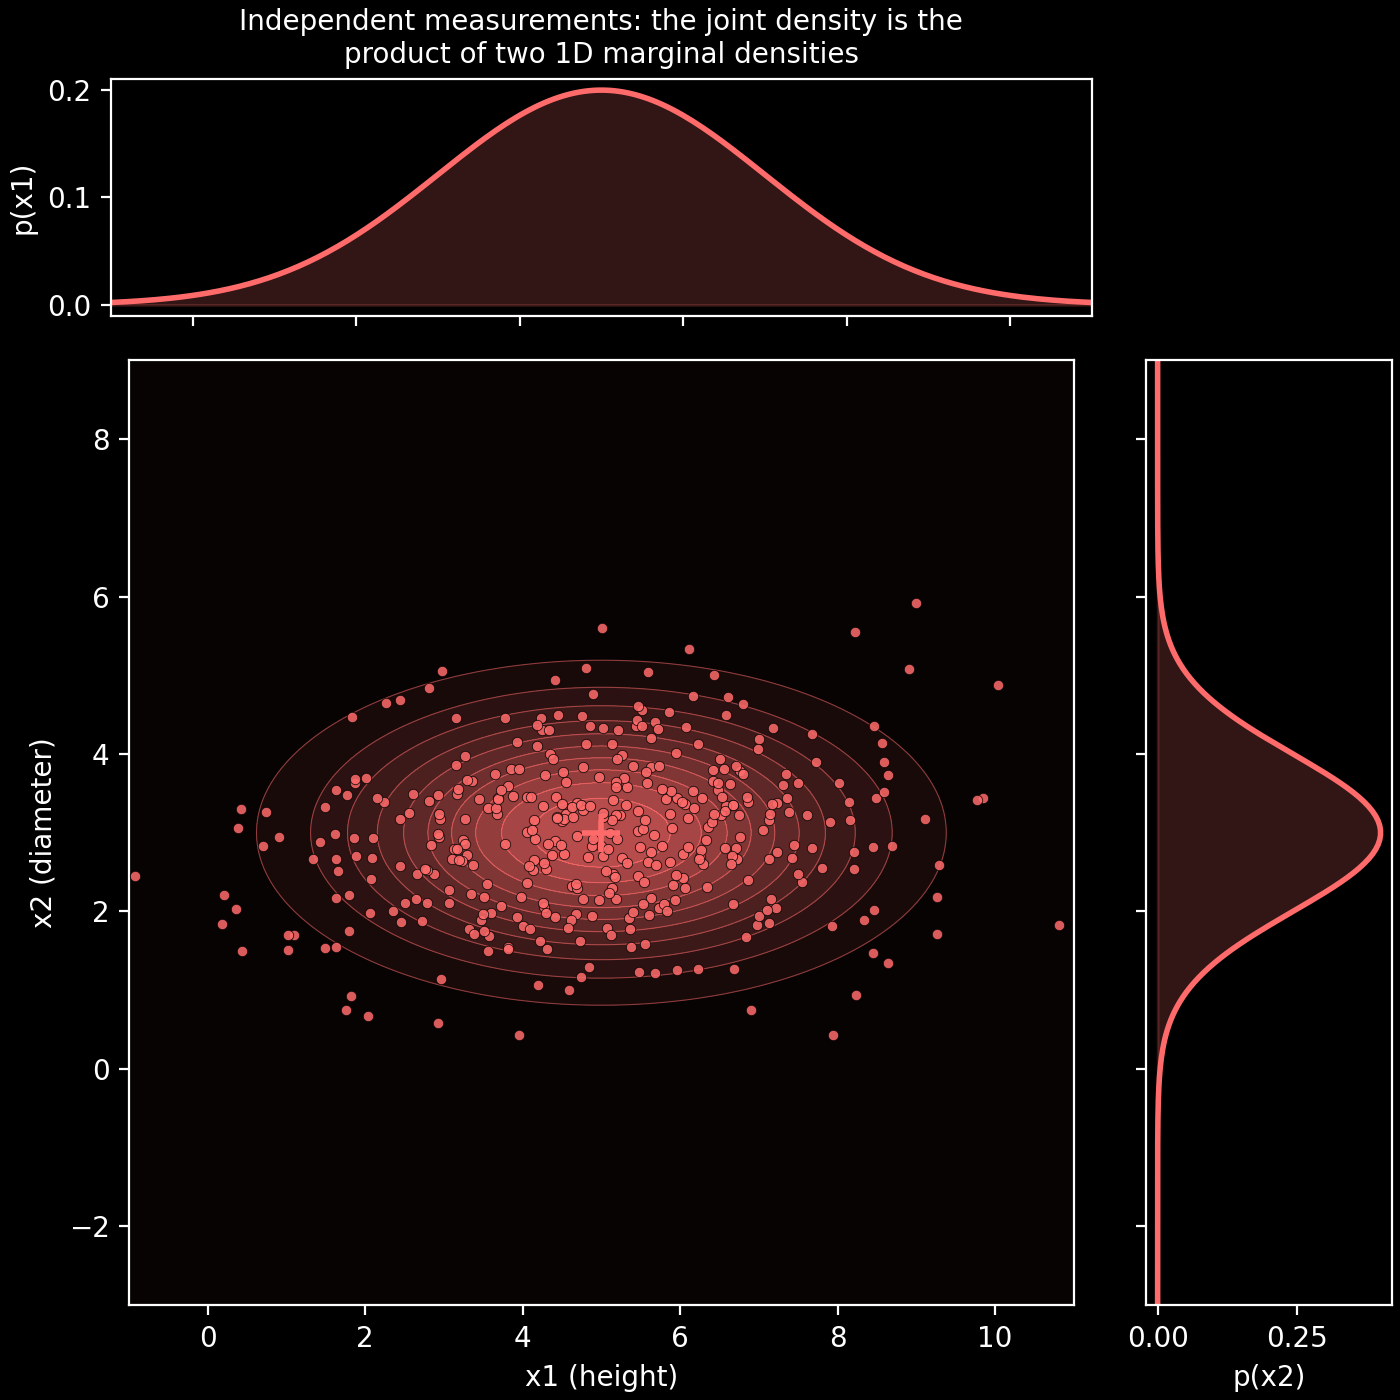
\includegraphics[width=0.6\textwidth]{../10_multivariate/outputs/diagonal_density_contours_dark.png}

\vspace{0.5em}
\small Equal-axis scatter of $(X_1, X_2)$, flanked by the two 1D marginal densities multiplied together above. Here $\sigma_1 = 2\sigma_2$, so the cloud is twice as wide as it is tall --- with no tilt, since the two measurements are independent.
\note{Point out the equal axis scaling --- without it, the shape of the cloud cannot be trusted. Ask students what would happen to this picture if X1 and X2 were correlated instead: the cloud would tilt. That is exactly the next topic.}
\end{frame}

\begin{frame}[c]{Correlated dimensions: entry by entry}
\textbf{Now suppose} taller biscuit tins also tend to be wider --- a single variance per dimension is no longer enough.

Let $v_i = X_i - \mu_i$ for each of $d$ measurements. The covariance matrix $\boldsymbol\Sigma$ is a $d \times d$ matrix of expected products:

\[
\boldsymbol\Sigma = \mathbb{E}\begin{pmatrix}
v_1^2 & v_1 v_2 & \cdots & v_1 v_d \\
v_2 v_1 & v_2^2 & \cdots & v_2 v_d \\
\vdots & \vdots & \ddots & \vdots \\
v_d v_1 & v_d v_2 & \cdots & v_d^2
\end{pmatrix}
\]

\textbf{Diagonal:} $\mathbb{E}[v_i^2] = \mathrm{Var}(X_i)$ --- the variance of each measurement, alone.

\textbf{Off-diagonal:} $\mathbb{E}[v_i v_j]$ --- positive means the two rise together, negative means one falls as the other rises, near zero means little relationship.
\note{This is the entry-by-entry picture behind equation 7.5. Each entry of this matrix is an expected value of a product of two (possibly the same) coordinates. The diagonal recovers the ordinary per-coordinate variance seen in the independent case; the off-diagonal entries are new --- they capture how pairs of coordinates move together. The next slide shows the compact notation mathematicians use to write this whole matrix at once.}
\end{frame}

\begin{frame}[c]{Reminder: outer products}
An \textbf{outer product} multiplies a column vector by a row vector, producing a matrix --- not a number.

\vspace{0.5em}
For a $d$-dimensional column vector $\mathbf{v}$:
\[
\mathbf{v}\mathbf{v}^T = \begin{pmatrix} v_1 \\ v_2 \\ \vdots \\ v_d \end{pmatrix} \begin{pmatrix} v_1 & v_2 & \cdots & v_d \end{pmatrix} = \begin{pmatrix} v_1^2 & v_1 v_2 & \cdots & v_1 v_d \\ v_2 v_1 & v_2^2 & \cdots & v_2 v_d \\ \vdots & \vdots & \ddots & \vdots \\ v_d v_1 & v_d v_2 & \cdots & v_d^2 \end{pmatrix}
\]

\vspace{0.5em}
\textbf{Shape check:} $(d\times 1)(1\times d) = (d\times d)$ --- the opposite of a dot product $\mathbf{v}^T\mathbf{v}$, which is $(1\times d)(d\times 1) = (1\times 1)$, a scalar.
\note{Students often confuse outer products with dot products, since both start from ``multiplying two vectors.'' The distinguishing feature is order: column times row (outer product) gives a matrix; row times column (dot product) gives a scalar. This d-by-d shape is exactly the shape of the covariance matrix --- no coincidence, since the next slide shows Sigma is literally built from outer products.}
\end{frame}

\begin{frame}[c]{Correlated dimensions: compact notation}
The matrix from the previous slides has a compact form, valid for any number of dimensions:
\[
\boldsymbol\Sigma = \mathbb{E}\left[(\mathbf{X}-\boldsymbol\mu)(\mathbf{X}-\boldsymbol\mu)^T\right]
\]

\vspace{0.5em}
\textbf{Why this works:} $(\mathbf{X}-\boldsymbol\mu)$ is a $d$-dimensional column vector; multiplying it by its own transpose is exactly the outer product from the previous slide, with $\mathbf{v} = \mathbf{X}-\boldsymbol\mu$.

\vspace{0.5em}
When every off-diagonal entry is zero, this reduces exactly to the independent case from earlier.
\note{This is equation 7.5 in its usual compact form. Point out explicitly that this is not a new idea --- it is shorthand for the entry-by-entry matrix and the outer-product shape just shown. (X - mu) is a column vector, and multiplying a column vector by its own transpose (an outer product) produces exactly the v_i v_j matrix from two slides back. When every off-diagonal entry is zero, this reduces exactly to equation 7.4, the independent case.}
\end{frame}

\begin{frame}[c]{Estimating $\boldsymbol\Sigma$ from data: the matrix $\mathbf{V}$}
Mean-center each sample: $\mathbf{v}^{(i)} = \mathbf{x}^{(i)} - \boldsymbol\mu = \left(v_1^{(i)}, v_2^{(i)}\right)$.

\vspace{0.5em}
Stack the centered samples as \emph{rows} of an $n \times 2$ matrix $\mathbf{V}$ --- the same row-per-sample layout \texttt{numpy}, \texttt{pandas}, and \texttt{scikit-learn} use:

\[
\mathbf{V} = \begin{pmatrix}
v_1^{(1)} & v_2^{(1)} \\
v_1^{(2)} & v_2^{(2)} \\
\vdots & \vdots \\
v_1^{(n)} & v_2^{(n)}
\end{pmatrix}
\quad\text{--- one row per sample, one column per coordinate}
\]
\note{This is the row-per-sample data matrix underlying equation 7.6. Each row is one mean-centered sample point; the superscript (i) picks the sample, the subscript picks the coordinate (height or diameter). Emphasize the shape: n rows because there are n samples, 2 columns because there are 2 measured quantities. This is exactly the layout of a pandas DataFrame or a numpy array you'd feed to scikit-learn --- one row per observation.}
\end{frame}

\begin{frame}[c]{Estimating $\boldsymbol\Sigma$ from data: the formula}
With $\mathbf{V}$ as on the previous slide, the covariance matrix is the averaged matrix product $\mathbf{V}^T\mathbf{V}$ --- equivalently, the average of $n$ outer products, one per sample:
\[
\boldsymbol\Sigma = \frac{1}{n}\mathbf{V}^T\mathbf{V} = \frac{1}{n}\sum_{i=1}^n \mathbf{v}^{(i)}\left(\mathbf{v}^{(i)}\right)^T = \frac{1}{n}\sum_{i=1}^n \begin{pmatrix} v_1^2 & v_1 v_2 \\ v_1 v_2 & v_2^2 \end{pmatrix}
\]

\vspace{0.5em}
Diagonal entries: average squared deviation of each coordinate. Off-diagonal: average product of the two coordinates --- the covariance.
\note{This is equation 7.6. V-transpose V and the sum of outer products are the same computation viewed two ways: multiplying V by its own transpose automatically sums, over all n rows, the outer product of that row with itself --- the same rank-1 outer product from the reminder slide, built from one sample's centered coordinates. Each entry of the sum uses the coordinates of one sample at a time: the diagonal entries average the squared deviation of each coordinate, and the off-diagonal entry averages the product of the two coordinates together.}
\end{frame}

\begin{frame}[c]{The general multivariate density}
\[
p(\mathbf{x}; \boldsymbol\mu, \boldsymbol\Sigma) = \frac{1}{(2\pi)^{d/2}|\boldsymbol\Sigma|^{1/2}} \exp\left(-\frac{1}{2}(\mathbf{x}-\boldsymbol\mu)^T \boldsymbol\Sigma^{-1}(\mathbf{x}-\boldsymbol\mu)\right)
\]

\vspace{0.5em}
\centering
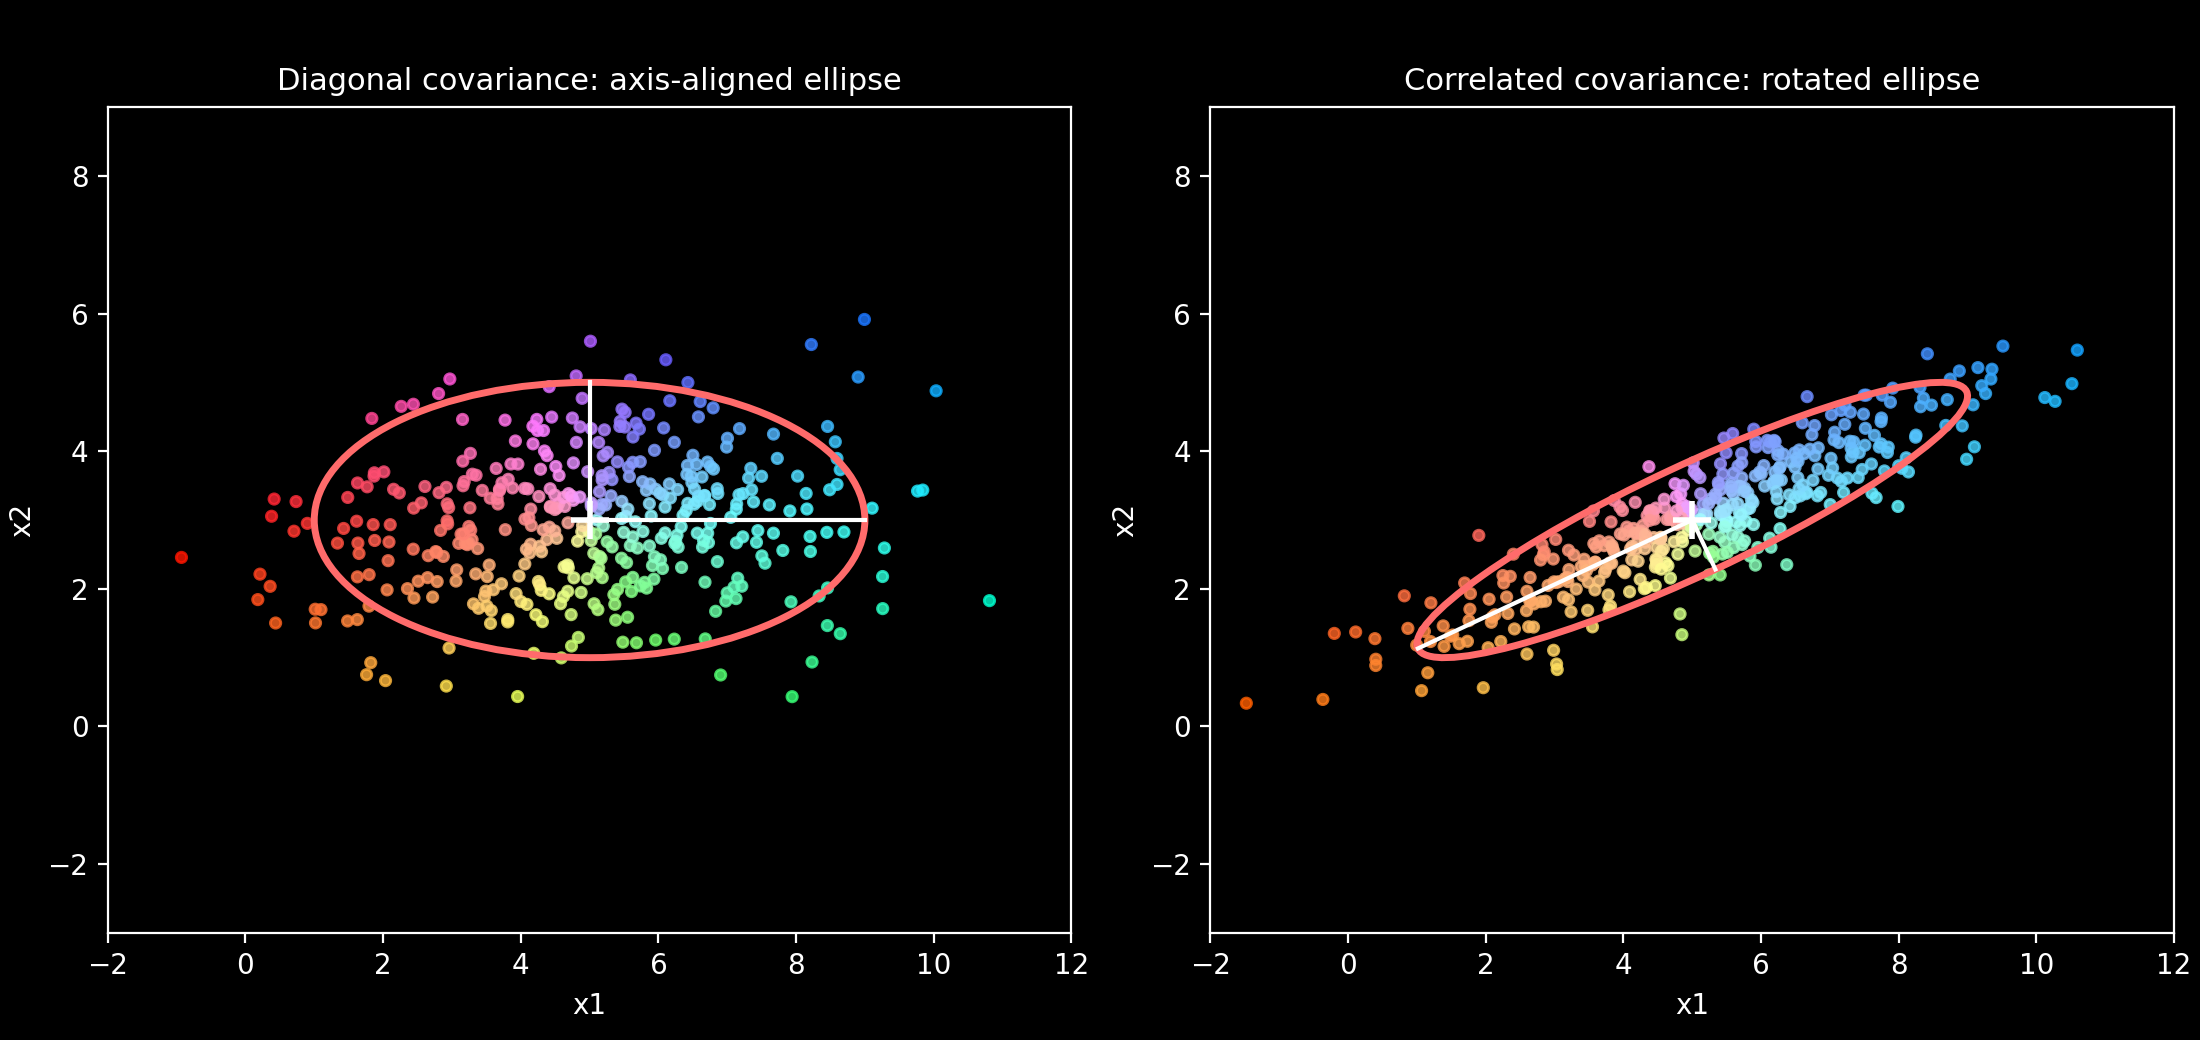
\includegraphics[width=0.75\textwidth]{../10_multivariate/outputs/covariance_ellipses_dark.png}

\small Left: diagonal covariance, axis-aligned (same as the independent case). Right: a positive off-diagonal covariance tilts the ellipse. Black lines mark the principal axes.
\note{This is equation 7.7. The geometric intuition in the figure matters more than the formula: a nonzero covariance tilts the ellipse. The principal axes drawn in black will be defined formally in a few slides --- for now just point out that they are not aligned with the coordinate axes on the right.}
\end{frame}

\begin{frame}[c]{A recipe for sampling correlated Gaussians}
Having seen how to estimate $\boldsymbol\Sigma$ from data, and using the ordinary sample mean for $\boldsymbol\mu$ --- here is a recipe for the opposite problem: generating correlated samples from any chosen $\boldsymbol\mu$ and $\boldsymbol\Sigma$.

\vspace{0.5em}
\textbf{Start with standard normal noise:}
\[
\mathbf{z} \sim \mathcal{N}(\mathbf{0}, \mathbf{I})
\]

\vspace{0.5em}
\textbf{Transform:} find a matrix $\mathbf{A}$ with $\mathbf{A}\mathbf{A}^T = \boldsymbol\Sigma$, then
\[
\mathbf{x} = \boldsymbol\mu + \mathbf{A}\mathbf{z}
\]

\vspace{0.5em}
Same reparameterization as $\sigma z + \mu$ from Lesson 6, with $\mathbf{A}$ replacing $\sigma$.
\note{This is equation 7.9. I is the identity matrix --- variance 1, no covariance, in every coordinate. The condition AA-transpose equals Sigma is what guarantees x ends up with the desired covariance. This is the multivariate version of the reparameterization trick from Lesson 6; students will see this same trick again when we discuss VAEs.}
\end{frame}

\begin{frame}[c]{Building $\mathbf{A}$: scale and rotate}
\textbf{Using two dimensions to visualize the idea} --- everything here extends directly to $d$ dimensions.

\vspace{0.5em}
\textbf{Scale matrix} $\mathbf{S}$ --- desired standard deviations on the diagonal:
\[
\mathbf{S} = \begin{pmatrix} \sigma_1 & 0 \\ 0 & \sigma_2 \end{pmatrix}
\]

\vspace{0.5em}
\textbf{Rotation} $\mathbf{R}(\theta)$ --- turns the axes toward the directions you want the ellipse to stretch:
\[
\mathbf{R}(\theta) = \begin{pmatrix} \cos\theta & -\sin\theta \\ \sin\theta & \cos\theta \end{pmatrix}
\]

\vspace{0.5em}
\textbf{Combine:} $\mathbf{A} = \mathbf{R}\mathbf{S}$
\note{This is equations 7.10 and 7.11. S scales standard deviations, not variances --- Sigma itself holds variances, which is why S is not squared. Two dimensions keep the matrices small enough to write out and visualize, but nothing here is special to 2D --- in d dimensions, S is still diagonal and R is still an orthogonal matrix built from d orthonormal columns. The directions R points the axes toward are called the principal component axes; the next slides show these are exactly the eigenvectors of Sigma.}
\end{frame}

\begin{frame}[c]{Why $\mathbf{R}^{-1} = \mathbf{R}^T$}
Write $\mathbf{R} = \begin{pmatrix} \mathbf{r}_1 & \mathbf{r}_2 \end{pmatrix}$ --- its columns are the new axis directions.

\vspace{0.5em}
\textbf{Each column has length 1:} \quad $\mathbf{r}_i^T \mathbf{r}_i = \cos^2\theta + \sin^2\theta = 1$

\vspace{0.5em}
\textbf{Different columns are perpendicular:} \quad $\mathbf{r}_1^T \mathbf{r}_2 = -\cos\theta\sin\theta + \sin\theta\cos\theta = 0$

\vspace{0.5em}
\textbf{So:}
\[
\mathbf{R}^T\mathbf{R} = \begin{pmatrix} \mathbf{r}_1^T\mathbf{r}_1 & \mathbf{r}_1^T\mathbf{r}_2 \\ \mathbf{r}_2^T\mathbf{r}_1 & \mathbf{r}_2^T\mathbf{r}_2 \end{pmatrix} = \begin{pmatrix} 1 & 0 \\ 0 & 1 \end{pmatrix} = \mathbf{I}
\]

\vspace{0.5em}
$\mathbf{R}^T\mathbf{R} = \mathbf{I}$ is exactly the definition of $\mathbf{R}^{-1} = \mathbf{R}^T$ --- the next slide confirms this holds the other way too.
\note{This confirms the R inverse equals R transpose claim used a moment ago. Unit-length, mutually perpendicular columns are called orthonormal; any matrix built from orthonormal columns satisfies R transpose R equals I. This orthonormal-columns property is what makes R a rotation (or reflection) rather than some other kind of linear transform, and it is the same property used later for higher-dimensional orthogonal matrices Q.}
\end{frame}

\begin{frame}[c]{Why $\mathbf{R}^{-1} = \mathbf{R}^T$, the other way}
The same argument works on \emph{rows} instead of columns: write $\mathbf{R} = \begin{pmatrix} \mathbf{r}_1^T \\ \mathbf{r}_2^T \end{pmatrix}$ using its rows this time.

\vspace{0.5em}
Rows are also unit length and perpendicular to each other, so:
\[
\mathbf{R}\mathbf{R}^T = \begin{pmatrix} \cos\theta & -\sin\theta \\ \sin\theta & \cos\theta \end{pmatrix}\begin{pmatrix} \cos\theta & \sin\theta \\ -\sin\theta & \cos\theta \end{pmatrix} = \begin{pmatrix} 1 & 0 \\ 0 & 1 \end{pmatrix} = \mathbf{I}
\]

\vspace{0.5em}
$\mathbf{R}^T\mathbf{R} = \mathbf{R}\mathbf{R}^T = \mathbf{I}$: since $\mathbf{R}$ is square, a left inverse is automatically a two-sided inverse.
\note{This is the other half of the R inverse equals R transpose argument. Because R is square, showing R transpose R equals I on the previous slide already guarantees R R transpose equals I too --- but it is worth confirming directly: the rows of R are the same unit vectors as its columns, just arranged differently, so the same cosine-squared-plus-sine-squared and cross-term cancellation argument applies. Both directions together are exactly the definition of a matrix inverse.}
\end{frame}

\begin{frame}[c]{Applying $\mathbf{A}$: scale first, then rotate}
Reading $\mathbf{A}\mathbf{z} = \mathbf{R}(\mathbf{S}\mathbf{z})$ right to left shows the actual order of operations:
\[
\mathbf{A}\mathbf{z} = \mathbf{R}\mathbf{S}\mathbf{z} = \mathbf{R}\underbrace{(\mathbf{S}\mathbf{z})}_{\text{scale first}}
\]

\vspace{0.5em}
\textbf{Scale first,} in the axis-aligned frame where scaling means something concrete --- stretching along a known direction --- and only then rotate into the orientation you actually want.

\vspace{0.5em}
\textbf{Analogy:} if getting from room A to room C means walking through room B first, retracing your steps means leaving room B, then room A --- not the other way around.

\vspace{0.5em}
\textbf{Confirming the covariance:} transposing a product reverses the order of its factors:
\[
\mathbf{A}\mathbf{A}^T = (\mathbf{R}\mathbf{S})(\mathbf{R}\mathbf{S})^T = \mathbf{R}\mathbf{S}\mathbf{S}^T\mathbf{R}^T = \mathbf{R}\mathbf{S}^2\mathbf{R}^T
\]
\note{Scaling after rotating would stretch the wrong directions, since the axes no longer line up with sigma-one and sigma-two. The underbrace makes the order concrete: Az first scales z by S, then rotates the result by R. The AA-transpose identity at the bottom confirms this order also produces the right covariance --- R S squared R transpose --- matching Sigma. Students who want the full matrix-shape argument for why (RS)^T = S^T R^T, not R^T S^T, can find it written out on the Canvas page.}
\end{frame}

\begin{frame}[c]{The recipe, visualized}
\centering
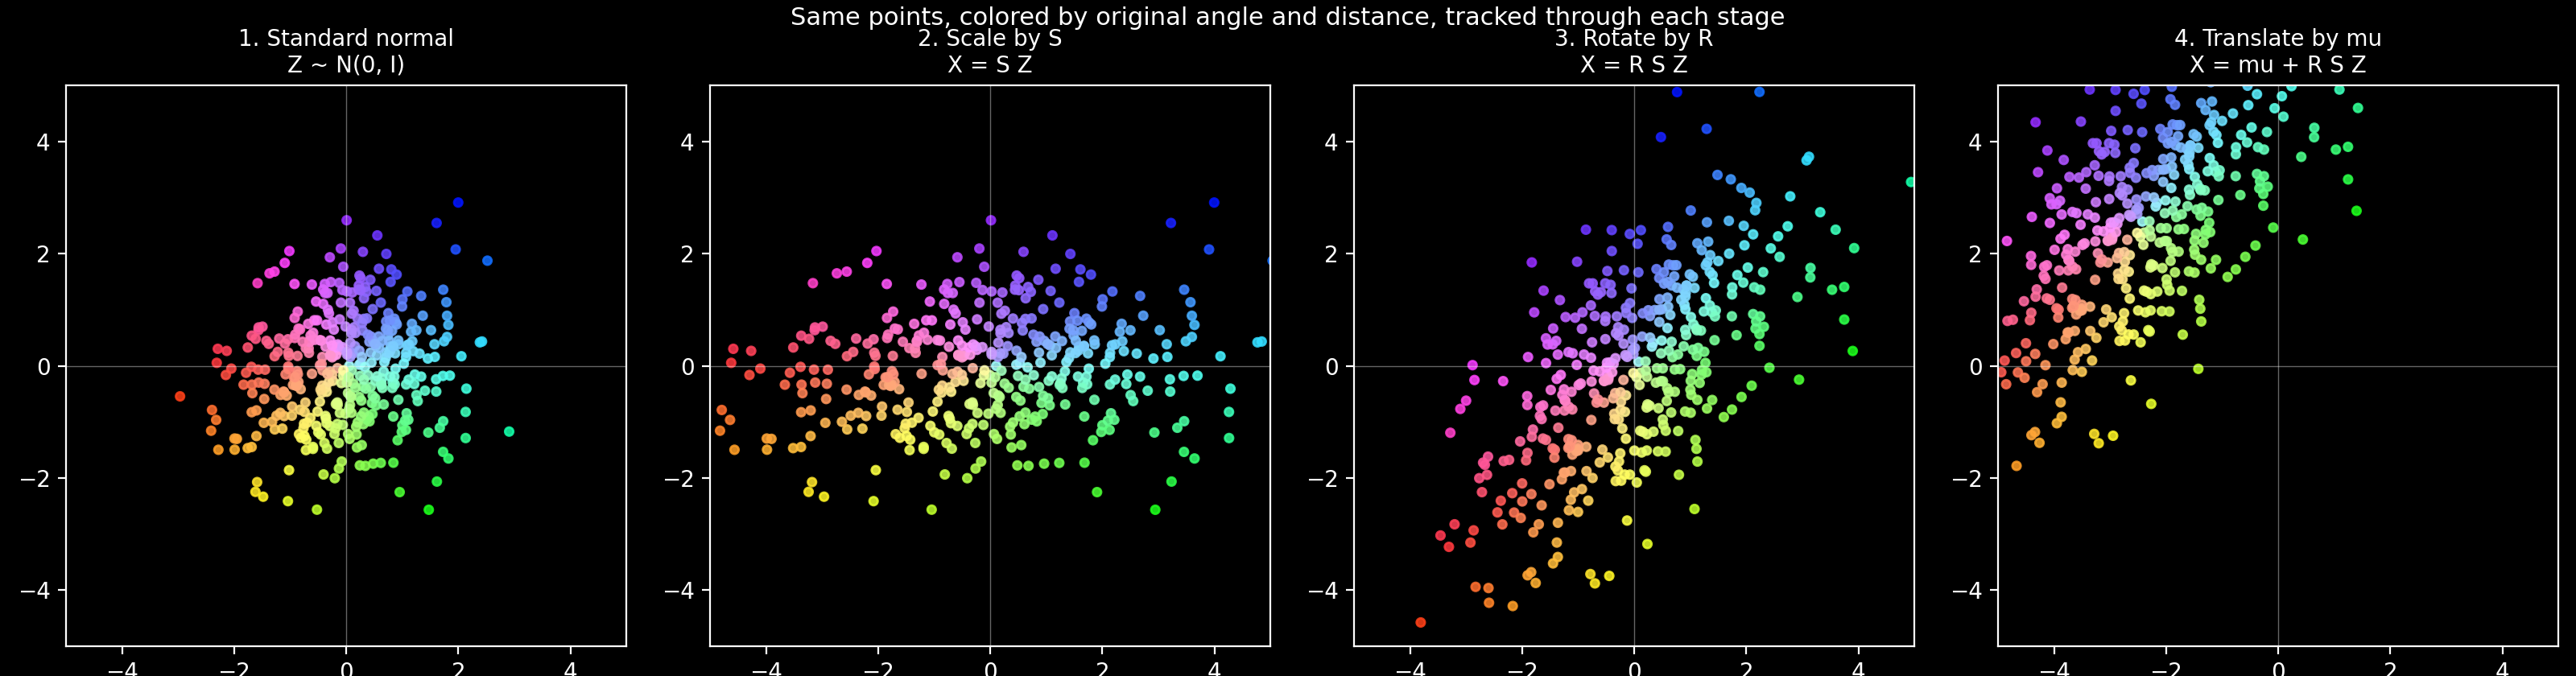
\includegraphics[width=0.9\textwidth]{../11_transform/outputs/transform_normal_dark.png}

\vspace{0.5em}
\small Standard-normal samples (1) are stretched by $\mathbf{S}$ (2), rotated by $\mathbf{R}$ (3), and shifted by $\boldsymbol\mu$ (4) --- producing a correlated Gaussian with a chosen center, spread, and orientation.
\note{This is Figure 7.3 from the page. Walk through the four panels in order and connect each to the equations from the last two slides: panel 2 is Sz, panel 3 is RSz, panel 4 adds mu. Points are colored by angle and distance from center so students can track individual points across the transformation.}
\end{frame}

\begin{frame}[c]{Undoing the recipe: whitening}
The recipe runs in reverse too: given correlated $\mathbf{x}$, undo each step to recover standard-normal $\mathbf{z}$.
\[
\mathbf{z} = \mathbf{S}^{-1}\mathbf{R}^T(\mathbf{x} - \boldsymbol\mu)
\]

\vspace{0.5em}
\centering
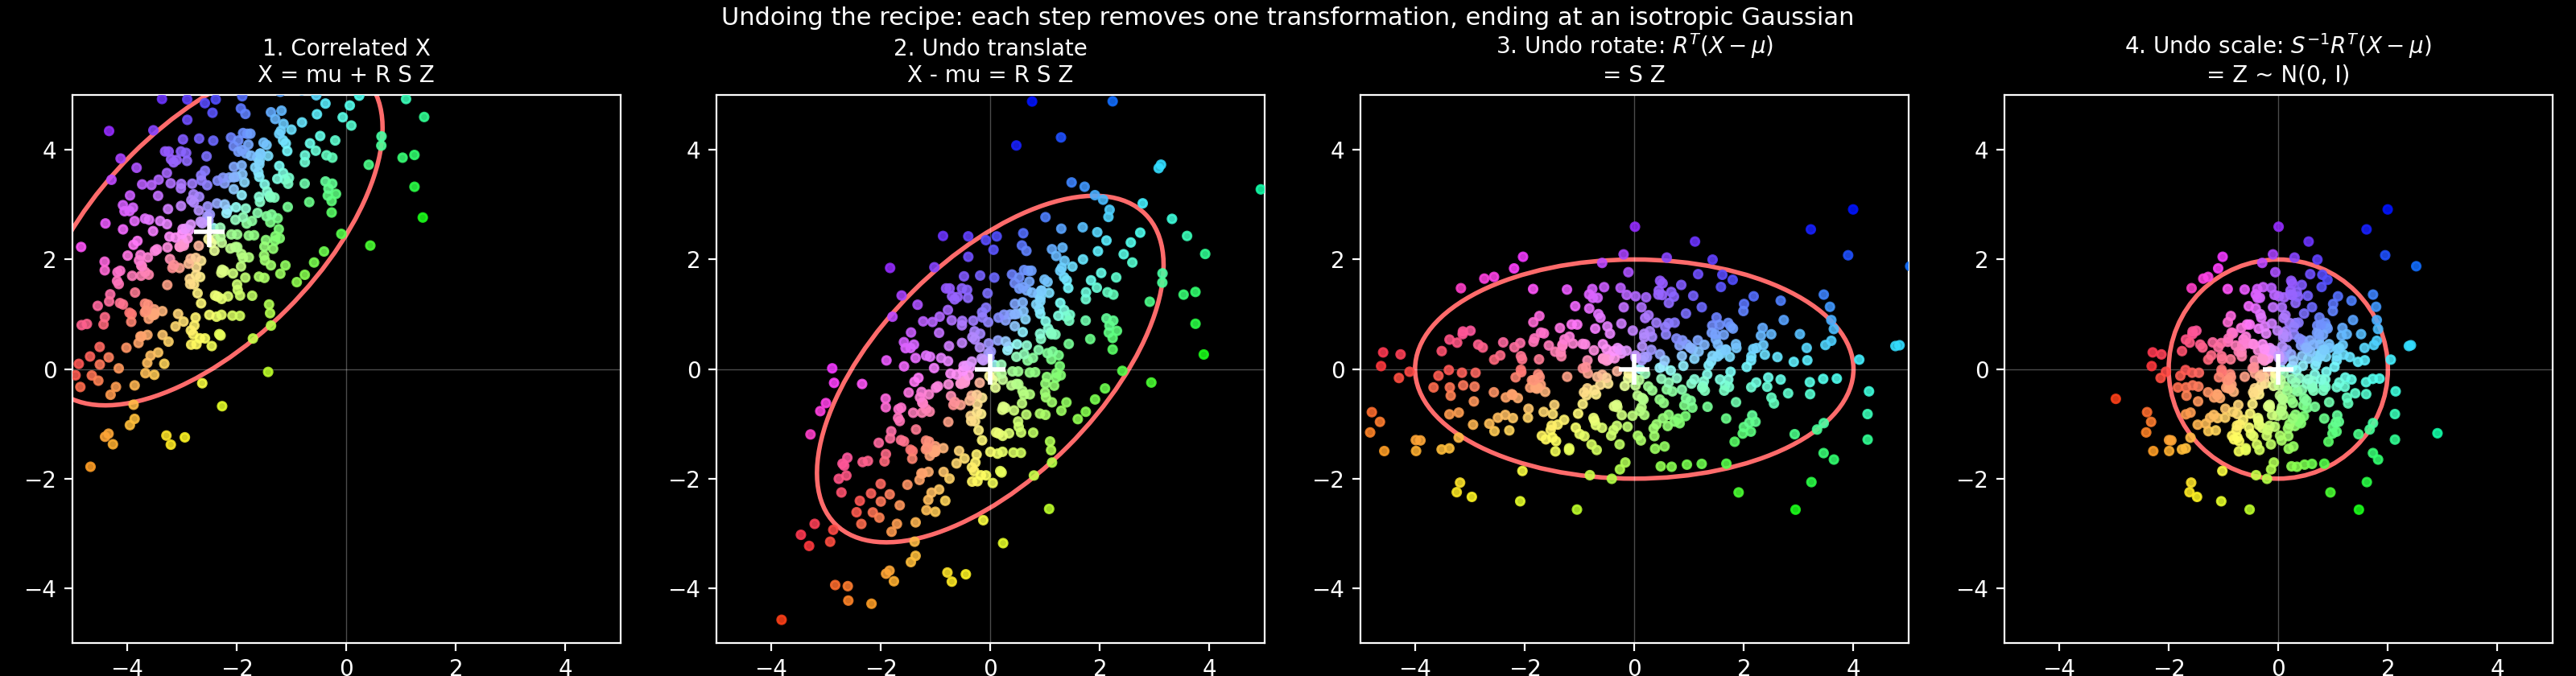
\includegraphics[width=0.9\textwidth]{../12_mahalanobis/outputs/whitening_recipe_dark.png}

\vspace{0.5em}
\small Undo the translation, then the rotation ($\mathbf{R}^T$), then the scale ($\mathbf{S}^{-1}$) --- the ellipse un-tilts and un-stretches at each step, ending at an isotropic circle.
\note{This is the exact reverse of the previous slide's recipe, using R inverse equals R transpose from a few slides back. This ``whitening'' transform is the bridge to Mahalanobis distance on the next slide: since S and R only rescale and rotate, the Euclidean distance of z from the origin in this standardized space is exactly the Mahalanobis distance of x from mu in the original space.}
\end{frame}

\begin{frame}[c]{Mahalanobis distance}
Ordinary (Euclidean) distance from $\boldsymbol\mu$ treats every direction equally --- misleading once the ellipse is tilted or stretched.

\vspace{0.5em}
\textbf{Mahalanobis distance} is exactly the Euclidean distance of the whitened point $\mathbf{z} = \mathbf{S}^{-1}\mathbf{R}^T(\mathbf{x}-\boldsymbol\mu)$ from the origin:
\[
D_M(\mathbf{x}) = \|\mathbf{z}\| = \sqrt{(\mathbf{x}-\boldsymbol\mu)^T \boldsymbol\Sigma^{-1} (\mathbf{x}-\boldsymbol\mu)}
\]

\vspace{0.5em}
\centering
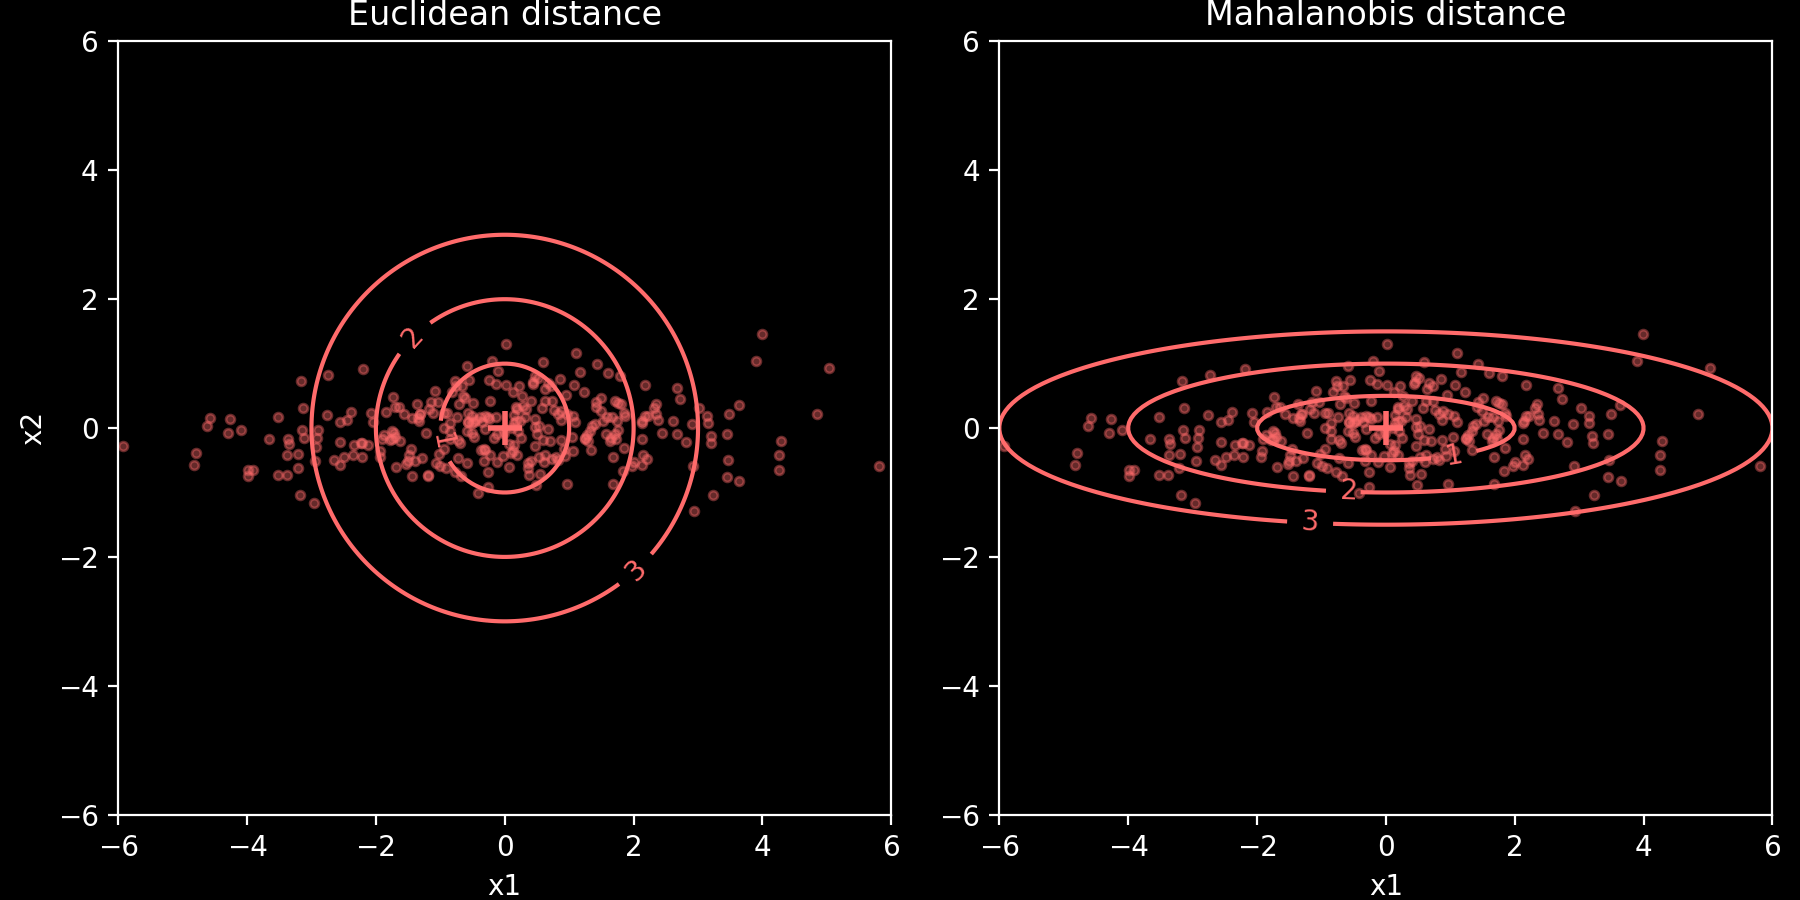
\includegraphics[width=0.75\textwidth]{../12_mahalanobis/outputs/mahalanobis_contours_dark.png}

\small Euclidean contours (left) are circles; Mahalanobis contours (right) are ellipses matching the data's spread --- a contour passes through equally ``typical'' points, not just equally distant ones.
\note{This is equation 7.8. The whitening transform from the previous slide is exactly what makes this equivalence hold: since S and R only rescale and rotate, z transpose z expands to (x minus mu) transpose Sigma inverse (x minus mu), because Sigma equals R S S transpose R transpose. A point a fixed Euclidean distance away along the long axis of the correlated ellipse is far more typical than the same distance along the short axis; Mahalanobis distance corrects for that by measuring in the whitened space instead.}
\end{frame}

\begin{frame}[c]{Principal component axes}
The directions $\mathbf{R}$ points toward are the \textbf{principal component axes} of $\boldsymbol\Sigma$ --- the directions of greatest and least spread, always perpendicular.

\vspace{0.5em}
Formally, these are the \textbf{eigenvectors} of $\boldsymbol\Sigma$; the \textbf{eigenvalues} give the variance along each direction ($\sigma_1^2, \sigma_2^2$).

\vspace{0.5em}
\[
\mathbf{S}\mathbf{S}^T = \begin{pmatrix} \sigma_1^2 & 0 \\ 0 & \sigma_2^2 \end{pmatrix}
\]

\vspace{0.5em}
\textbf{Key idea:} every covariance matrix is really a diagonal one (independent measurements), viewed from a rotated angle.
\note{Point back to the tilted ellipse from the correlated-dimensions figure earlier in the lesson: rotating the coordinate system to line up with these black principal axes would turn the ellipse back into an axis-aligned one, exactly like the independent case, just with different variances along each axis. In higher dimensions this rotation generalizes to an orthogonal matrix, which also includes reflections --- that distinction rarely matters for a Gaussian, since reflecting through a principal axis leaves the ellipse unchanged.}
\end{frame}

\begin{frame}[fragile]{Fitting a Gaussian is PCA}
Fitting a multivariate Gaussian means estimating $\boldsymbol\mu$ and $\boldsymbol\Sigma$.

\vspace{0.5em}
\textbf{The mean} is just the sample mean, exactly as in the 1D case --- only now each $\mathbf{x}_i$ is a vector:
\[
\hat{\boldsymbol\mu} = \frac{1}{n}\sum_{i=1}^n \mathbf{x}_i
\]

\vspace{0.5em}
\textbf{The covariance} is $\hat{\boldsymbol\Sigma} = \frac{1}{n}\mathbf{V}^T\mathbf{V}$, shown a few slides back.

\vspace{0.5em}
\textbf{What you usually want:} the principal axes and variances along them --- the eigenvectors and eigenvalues of $\boldsymbol\Sigma$.

\begin{lstlisting}[language=Python]
eigenvalues, eigenvectors = numpy.linalg.eigh(Sigma)
std_devs = numpy.sqrt(eigenvalues)  # diagonal of S
R = eigenvectors  # columns = axes
\end{lstlisting}
\note{This is equation 7.12, paired with equation 7.6 shown earlier. The mean formula is new here but should feel unsurprising: it is the same arithmetic-mean idea from Lesson 6, just applied one vector at a time instead of one number at a time. Warn students to read the eigh output carefully: eigenvalues come back as variances, not standard deviations, so take the square root to get S. This decomposition --- splitting Sigma into a rotation and a scale --- is exactly the algorithm known as PCA. Proving that these eigenvectors maximize captured variance is optional for this course.}
\end{frame}

\begin{frame}[c]{Eigenfaces: a generative model for images}
Everything above still works when each ``point'' is an entire image.

\vspace{0.5em}
\begin{itemize}
    \item Flatten a grayscale face photo into one long vector $\mathbf{x}$ --- one entry per pixel
    \item A collection of faces becomes a cloud of points in a very high-dimensional space
    \item Fit a multivariate Gaussian using nothing more than the mean and covariance formulas above
\end{itemize}

\vspace{0.5em}
This is the idea behind \textbf{eigenfaces} (Turk and Pentland, 1991).
\note{Emphasize the dimensionality jump: thousands of pixels instead of two coordinates, but the same equations 7.6 and 7.12 apply unchanged. This is a good moment to check whether students see why nothing about the math required exactly two dimensions.}
\end{frame}

\begin{frame}[c]{Mean face, eigenfaces, and variance explained}
\centering
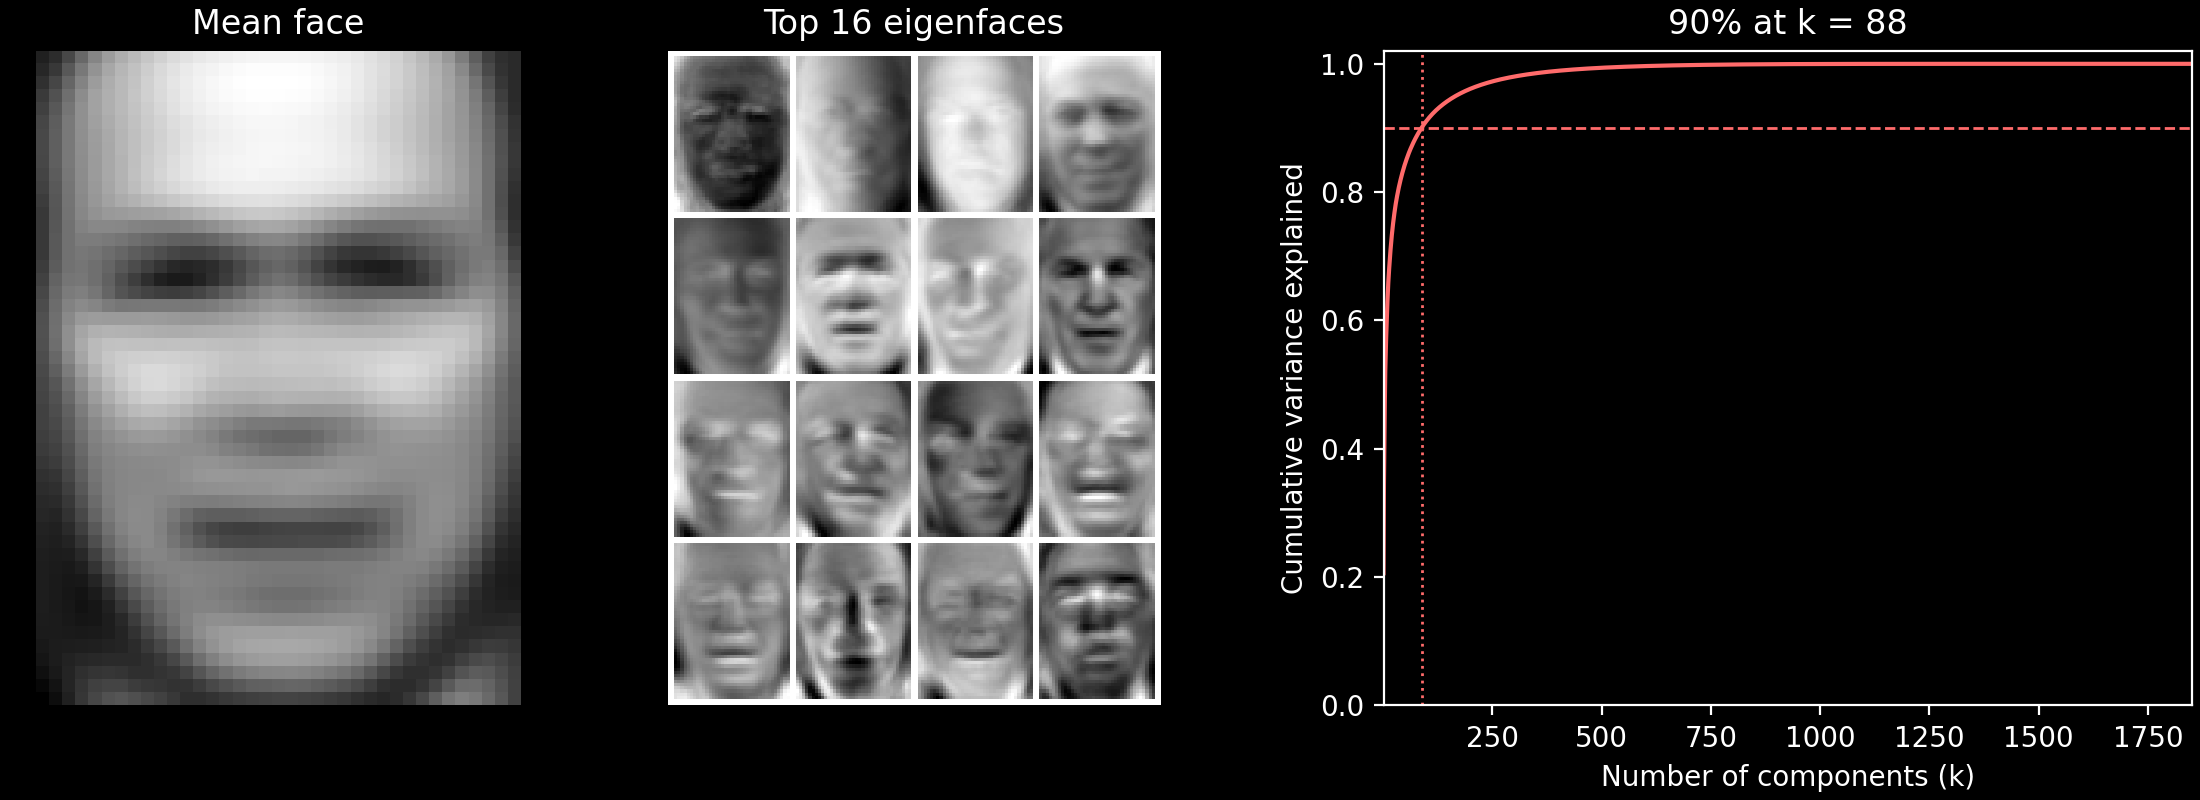
\includegraphics[width=0.95\textwidth]{../13_eigenfaces/outputs/eigenfaces_summary_dark.png}

\vspace{0.5em}
\small Left: the mean face $\hat{\boldsymbol\mu}$. Middle: the top 16 eigenfaces --- the principal axes of $\boldsymbol\Sigma$, reshaped back into images. Right: cumulative variance explained.
\note{Each eigenface's sign and scale are arbitrary --- only the spatial pattern of light and dark it captures is meaningful, which is why each is normalized independently for display. The eigenfaces with the largest variance capture the dominant patterns of variation across the dataset: a furrowed brow, a shift in lighting, a wider jaw.}
\end{frame}

\begin{frame}[c]{Sampling new faces}
Same sampling recipe from equation 7.9, applied to images:
\[
\mathbf{z} \sim \mathcal{N}(\mathbf{0}, \mathbf{I}), \qquad \mathbf{x} = \hat{\boldsymbol\mu} + \mathbf{A}\mathbf{z}
\]

\vspace{0.5em}
Each entry of $\mathbf{z}$ is a random weight used to create a mixture of the eigenfaces. Adding the weighted eigenfaces to the mean face produces a new synthetic face.

\vspace{0.5em}
\textbf{In practice:} keep only the first few dozen or hundred eigenfaces (largest variance) --- the rest mostly capture noise.

\vspace{0.5em}
This is a genuine \textbf{generative model}: sampling produces new examples, not just describing existing ones.
\note{This is the first point in the course where a model actually generates new, never-seen data by sampling a latent z and transforming it into data space. Faces generated this way tend to look blurry and averaged-out --- flag that VAEs, GANs, and diffusion models, later in the course, replace this single Gaussian with something far richer, but the sample-a-latent-then-transform idea is exactly the same one introduced here.}
\end{frame}

\begin{frame}[c]{Sampled faces vs. real faces}
\centering
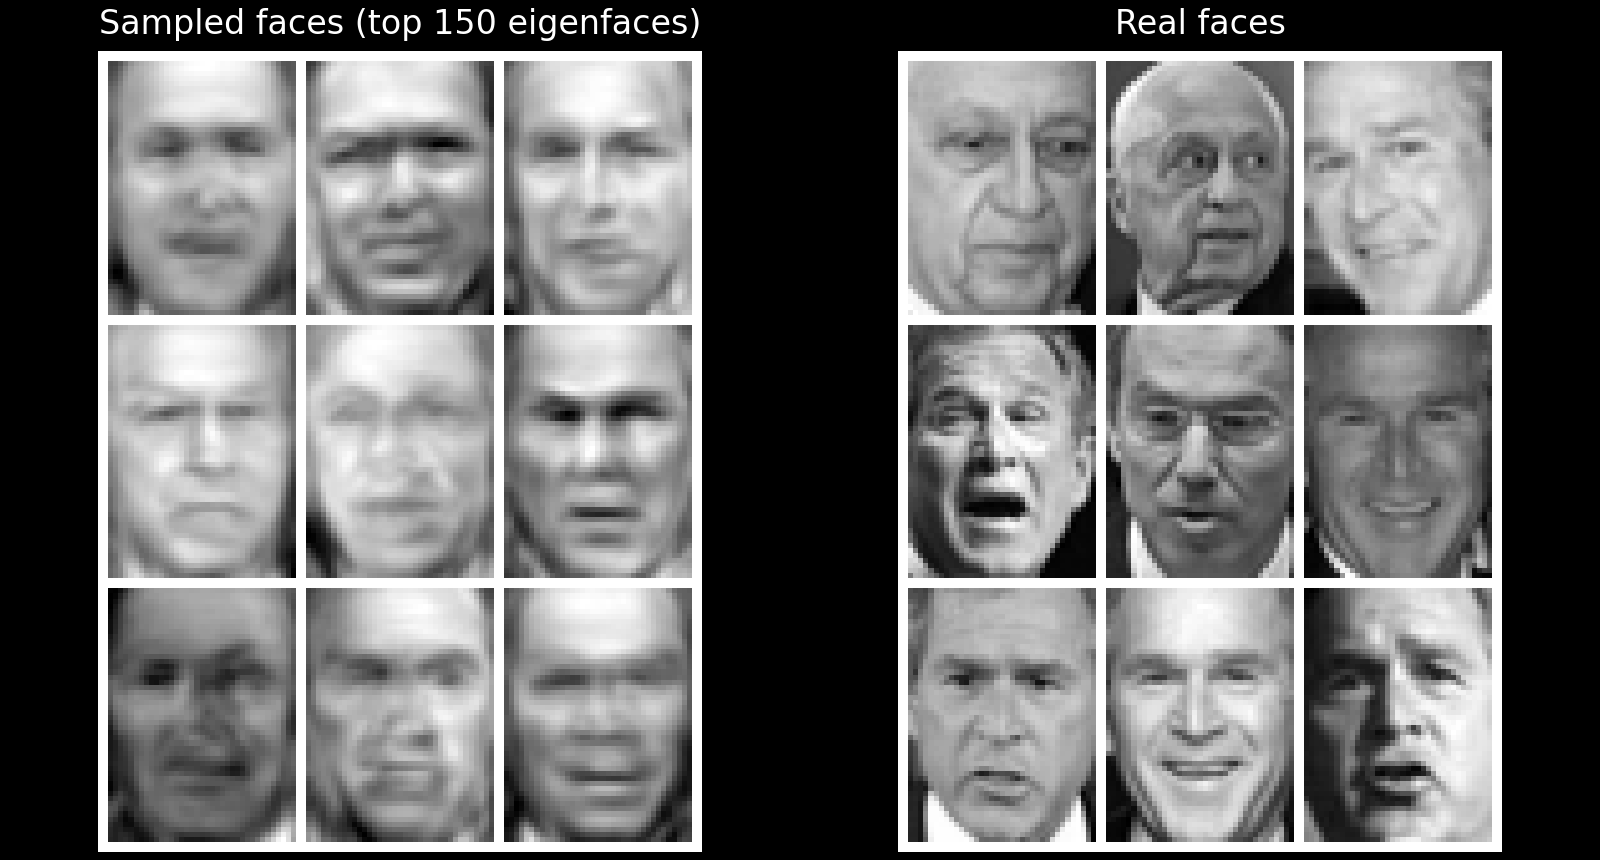
\includegraphics[width=0.85\textwidth]{../13_eigenfaces/outputs/sampled_faces_grid_dark.png}

\vspace{0.5em}
\small Left: nine faces sampled using only the top 150 eigenfaces ($\mathbf{z} \sim \mathcal{N}(\mathbf{0},\mathbf{I})$, $\mathbf{x} = \hat{\boldsymbol\mu} + \mathbf{R}(\mathbf{S}\mathbf{z})$), with $\mathbf{z}$ truncated to $\pm 0.8$ standard deviations so every sample stays in the dense, realistic-looking part of the distribution instead of the noisier tails. Right: nine real faces from the dataset, for comparison.
\note{The fitted mean, top-150 eigenfaces ($\mathbf{R}$), and their standard deviations ($\mathbf{S}$) are saved once to eigenfaces\_basis.npz so later demos can sample without recomputing the eigendecomposition. Truncating z is the same ``truncation trick'' used in GANs like BigGAN and StyleGAN: clipping the latent to a smaller range trades away some diversity in exchange for consistently plausible-looking samples, since draws far out in the tails of z tend to produce faces that look noisy or malformed. Point out what the comparison still shows even after truncation: the sampled faces are recognizably face-shaped --- eyes, nose, mouth, jawline all land in roughly the right places --- but look soft, symmetric, and averaged compared to the sharp, idiosyncratic real photos on the right. That blurriness is the direct consequence of keeping only 150 of nearly 1850 possible directions of variation and treating them as jointly Gaussian; it is exactly the limitation VAEs, GANs, and diffusion models are built to fix.}
\end{frame}

\begin{frame}[c]{PCA for dimension reduction}
Each face is a point in a 1850-pixel space --- far too many dimensions to plot or reason about directly.

\vspace{0.5em}
\textbf{Dimension reduction:} keep only the coordinates along the top few principal axes, and drop the rest.

\vspace{0.5em}
Projecting onto just the \textbf{top 2} eigenfaces gives every face a $(\text{PC1}, \text{PC2})$ score --- two numbers standing in for 1850 pixel values:
\[
\text{score} = \mathbf{v}^T \begin{pmatrix} \mathbf{r}_1 & \mathbf{r}_2 \end{pmatrix}
\]

\vspace{0.5em}
Nearby scores should belong to similar-looking faces --- the next slide checks whether that is actually true.
\note{This reframes the eigenfaces summary slide from a different angle: instead of asking what the eigenfaces look like, ask what happens if you throw away every coordinate except the top 2. v is the mean-centered pixel vector for one face, and r1, r2 are its first two eigenfaces (principal axes). The claim that nearby scores mean similar-looking faces is exactly what the grid visualization on the next slide tests directly.}
\end{frame}

\begin{frame}[c]{Visualizing the top 2 dimensions}
\centering
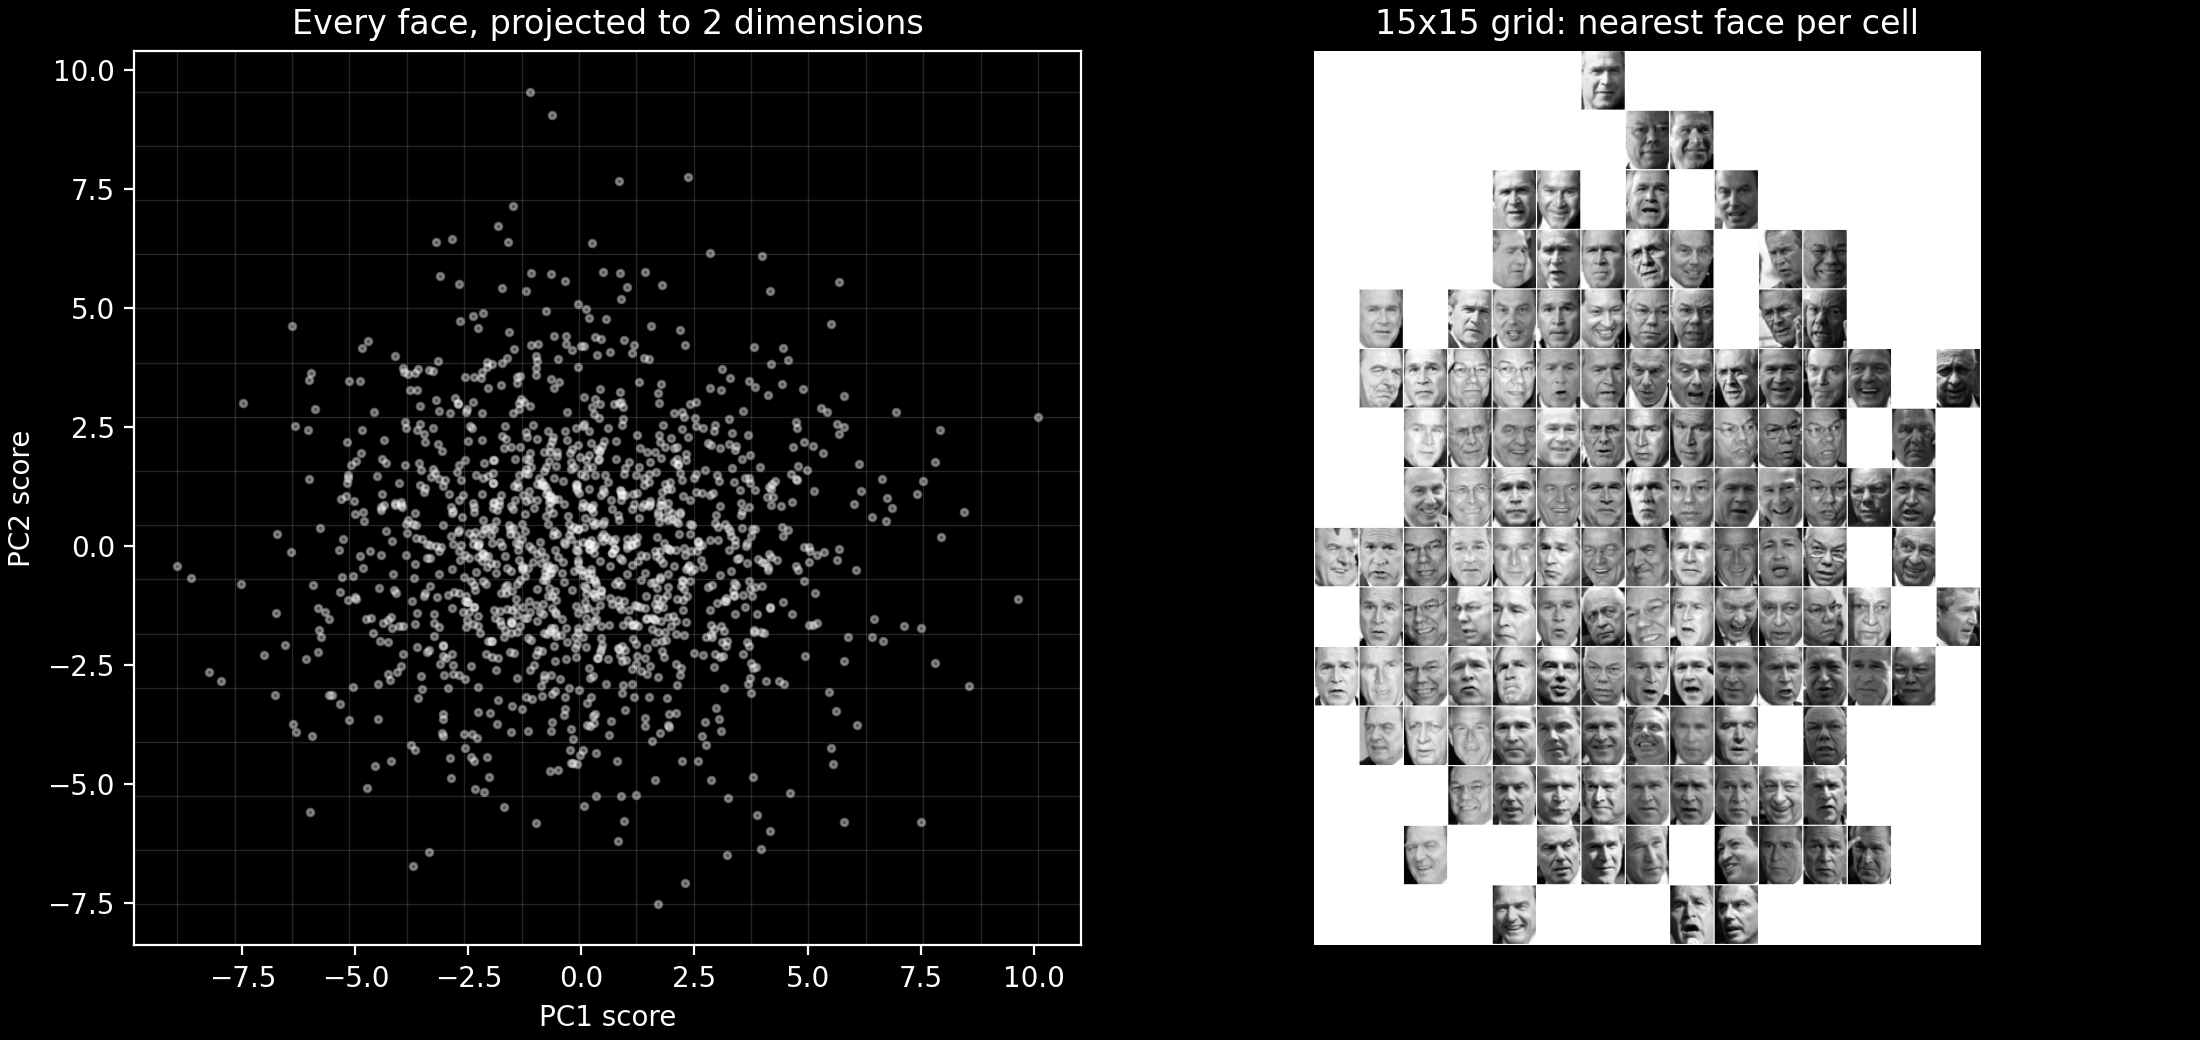
\includegraphics[width=0.95\textwidth]{../13_eigenfaces/outputs/pca_face_grid_dark.png}

\vspace{0.5em}
\small Left: every face's (PC1, PC2) score, with a $15\times15$ grid overlaid. Right: the face closest to each grid cell's center --- blank where no face landed in that cell.
\note{This is the direct test of the previous slide's claim. Walk left to right and top to bottom across the grid on the right: pose, lighting, and expression should change smoothly, since nearby cells are nearby points in PC1-PC2 space. Blank cells are simply grid cells no face happened to land in --- the scores cluster in a roughly circular cloud around the mean, so the corners of the square grid are often empty. This is the same nearest-point-per-grid-cell idea used to visualize any 2D embedding, not just PCA.}
\end{frame}

\begin{frame}[c]{Beyond PCA: other ways to see your data}
PCA is not the only way to compress data down to 2 dimensions for visualization --- and it has a real limitation: it only looks for \textbf{straight-line} directions of spread.

\vspace{0.5em}
Two popular alternatives instead try to preserve which points are \textbf{near each other}, even if that means bending the data into a different shape:
\begin{itemize}
    \item \textbf{UMAP} --- Uniform Manifold Approximation and Projection
    \item \textbf{t-SNE} --- t-distributed Stochastic Neighbor Embedding
\end{itemize}

\vspace{0.5em}
Both are useful for exploring whether your data has clusters or structure that a straight-line method like PCA might miss.
\note{This is an optional side note, not a formal derivation --- the goal is just for students to recognize these two names and know roughly what problem they solve. PCA's straight-line limitation matters when the true structure of the data is curved: think of data lying along a spiral, where any straight-line projection mixes together points that are actually far apart along the spiral. UMAP and t-SNE both prioritize local neighborhoods --- if two points are close in the original space, they try to keep them close in 2D, at the cost of no longer meaning anything by absolute distances or directions in the embedding.}
\end{frame}

\begin{frame}[c]{UMAP: same faces, a different embedding}
\centering
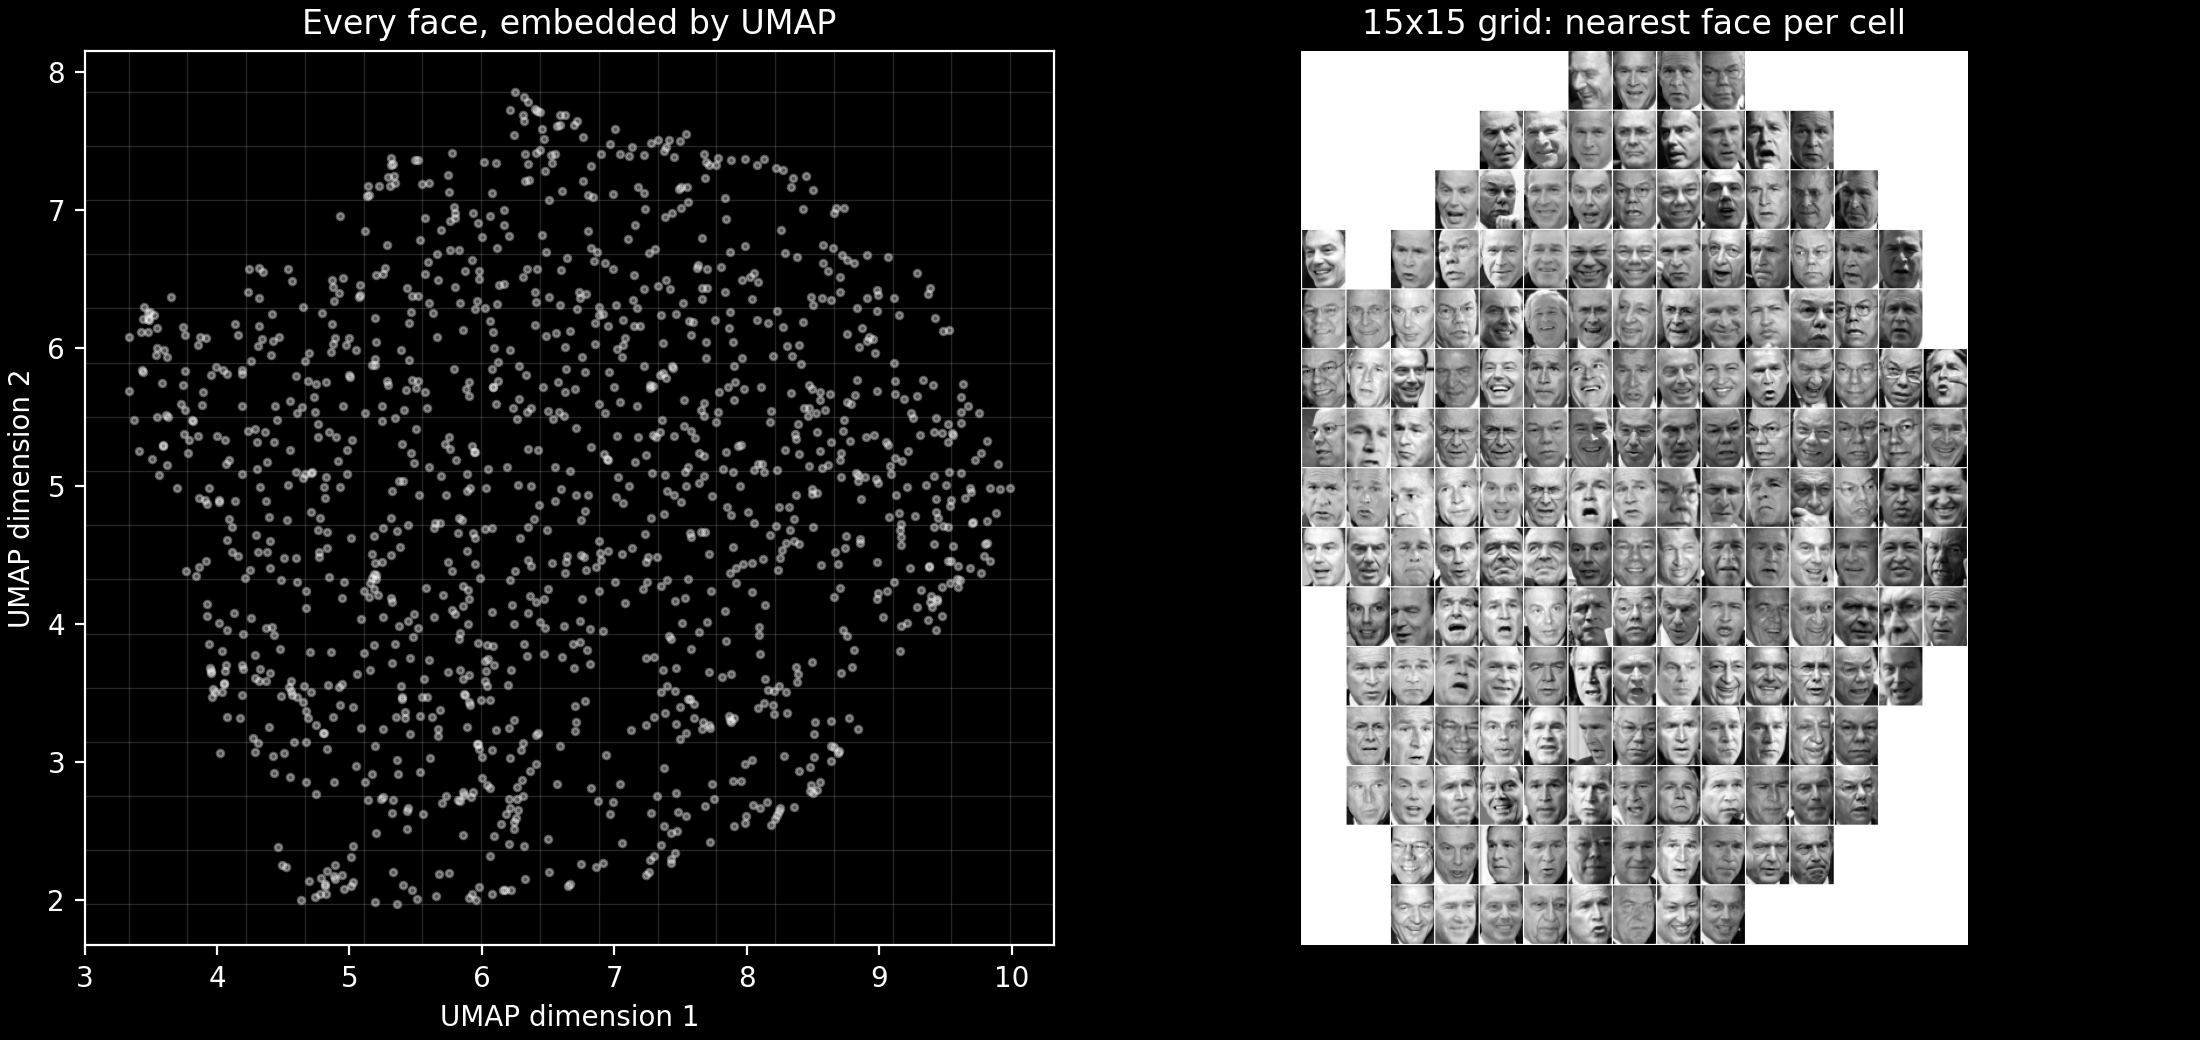
\includegraphics[width=0.95\textwidth]{../13_eigenfaces/outputs/umap_face_grid_dark.png}

\vspace{0.5em}
\small The same $15\times15$ nearest-face-per-cell grid, but the 2D coordinates come from UMAP instead of the top 2 principal components.
\note{Compare directly against the PCA grid a few slides back: UMAP tends to pack faces into a denser, more tightly clustered arrangement, since it is actively trying to keep neighboring faces close together rather than just capturing the two directions of greatest overall variance. The PC1/PC2 axis labels no longer apply here --- UMAP's two output dimensions do not correspond to any single interpretable direction in pixel space, only to relative closeness.}
\end{frame}

\begin{frame}[c]{t-SNE: same faces, another embedding}
\centering
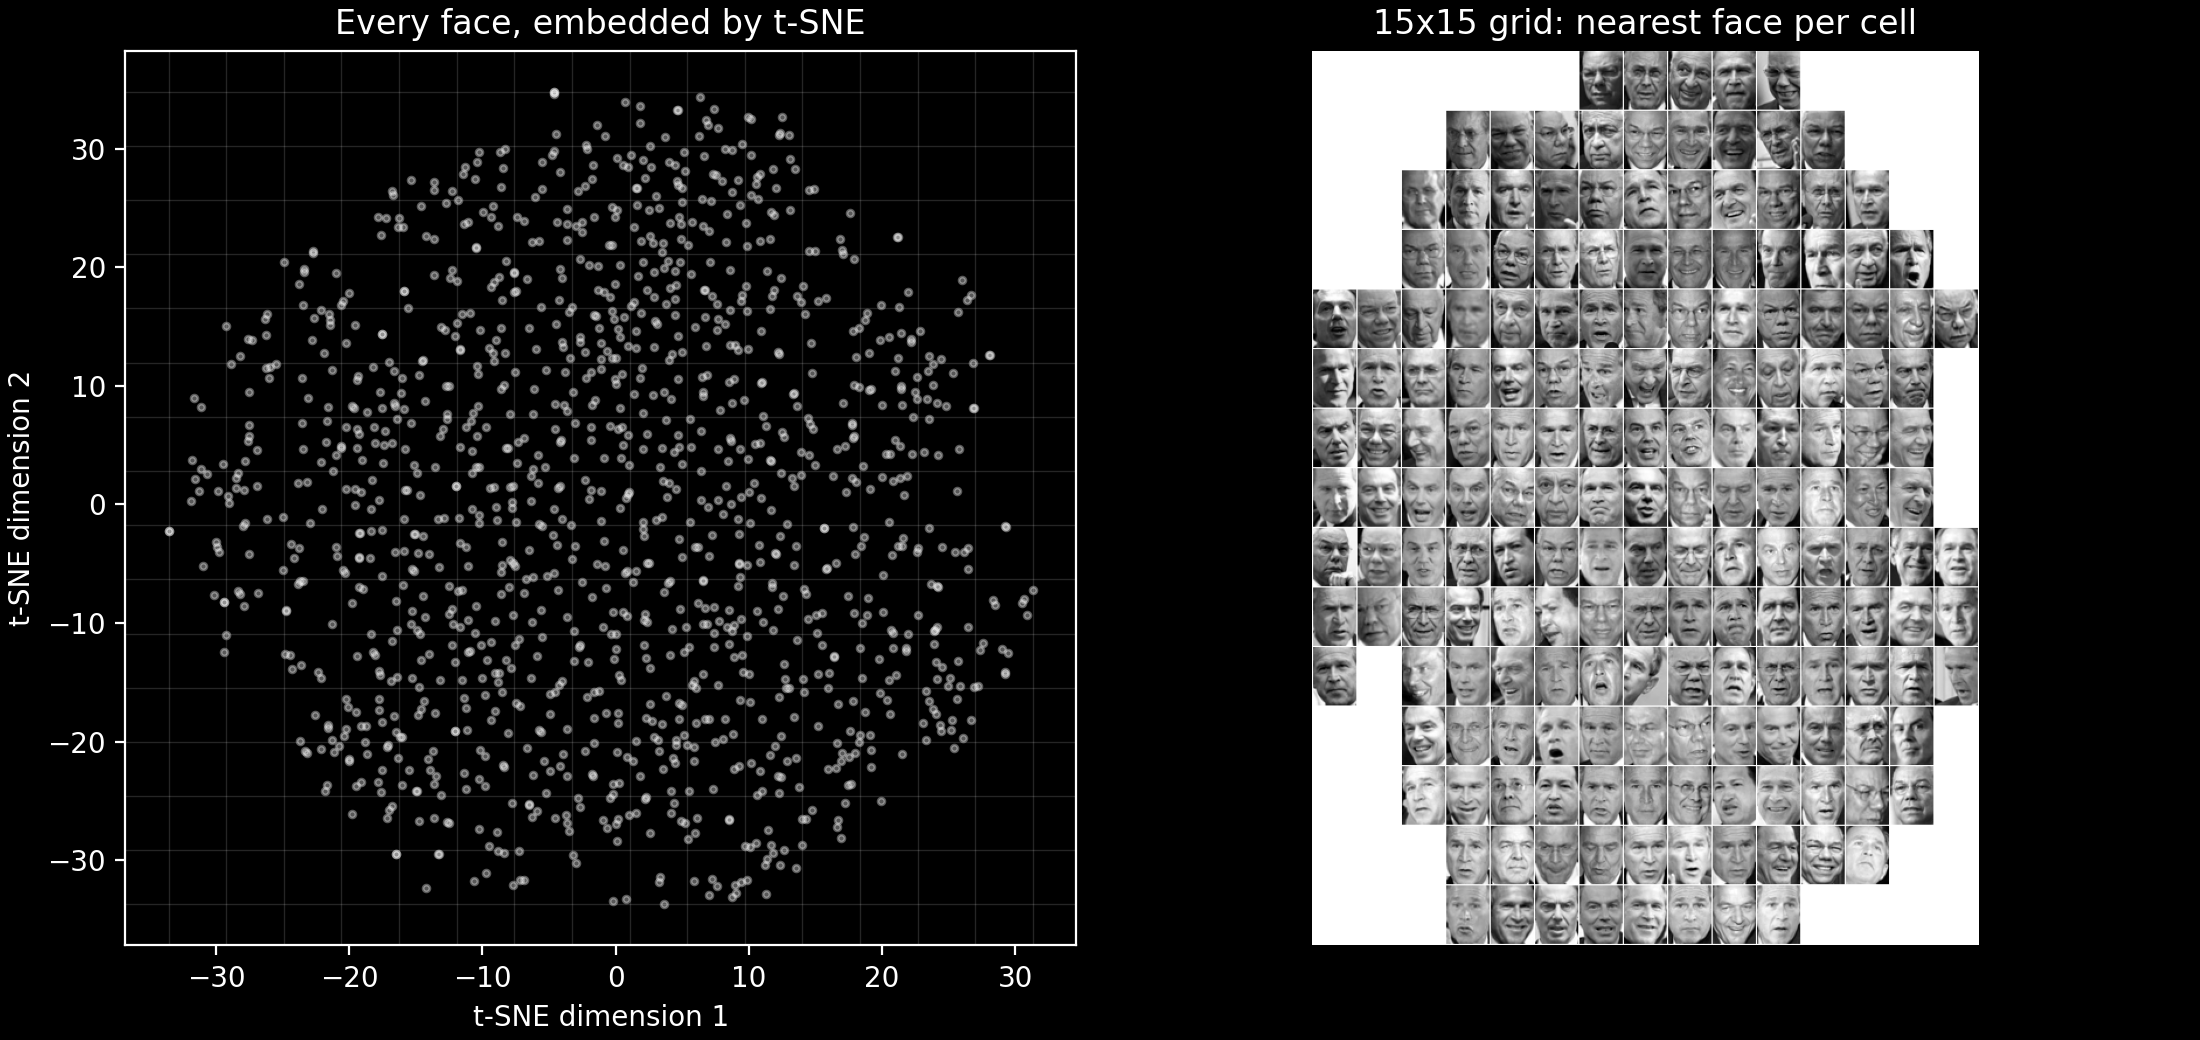
\includegraphics[width=0.95\textwidth]{../13_eigenfaces/outputs/tsne_face_grid_dark.png}

\vspace{0.5em}
\small The same $15\times15$ nearest-face-per-cell grid, using t-SNE's 2D coordinates instead.
\note{t-SNE, like UMAP, has no fixed global axes --- only relative neighborhoods are meaningful, and even the overall shape or size of clusters can be misleading (a well-known caveat with t-SNE). Compare all three grids (PCA, UMAP, t-SNE) side by side if time allows: the same underlying faces get rearranged quite differently depending on which method chose the 2D layout. The practical takeaway for students: PCA is fast, exact, and interpretable, but UMAP and t-SNE are often better at revealing cluster structure hiding in high-dimensional data.}
\end{frame}

\begin{frame}[c]{Coming up next}
\textbf{Next:} Tool Use, Retrieval, and Agentic Loops.

\vspace{1em}
\textbf{Further reading:}
\begin{itemize}
    \item PRML (Bishop), Section 2.3
    \item 3Blue1Brown: Linear transformations and matrices
    \item Gilbert Strang, MIT 18.06 --- Lectures 1--3 and 21 (eigenvalues and eigenvectors)
    \item Turk and Pentland, ``Eigenfaces for Recognition,'' 1991
    \item McInnes, Healy, and Melville, ``UMAP: Uniform Manifold Approximation and Projection,'' 2018
    \item van der Maaten and Hinton, ``Visualizing Data using t-SNE,'' 2008
\end{itemize}
\note{Today covered independent and correlated covariance, Mahalanobis distance, the scale-rotate-shift sampling recipe, principal component axes, eigenfaces as a first generative model, PCA for dimension reduction, and UMAP/t-SNE as alternative embeddings. The linear algebra refresher on the Canvas page links to Strang's full lecture series if vectors, matrices, or eigenvectors still feel unfamiliar.}
\end{frame}

\end{document}
